% Add these packages to the preamble:
%
% \usepackage{graphicx}
% \usepackage{booktabs}
% \usepackage{siunitx}
% \usepackage{tabularx}
% \usepackage{subcaption}
%
% Load generated commands:
% % Automatically generated.
\newcommand{\TheoreticalIneffectiveRate}{36.716\%}
\newcommand{\RecoveredFaultInput}{\texttt{0x5a}}
\newcommand{\RecoveredRTK}{\texttt{b3ed58adabab101d}}


\begin{figure}[t]
    \centering
    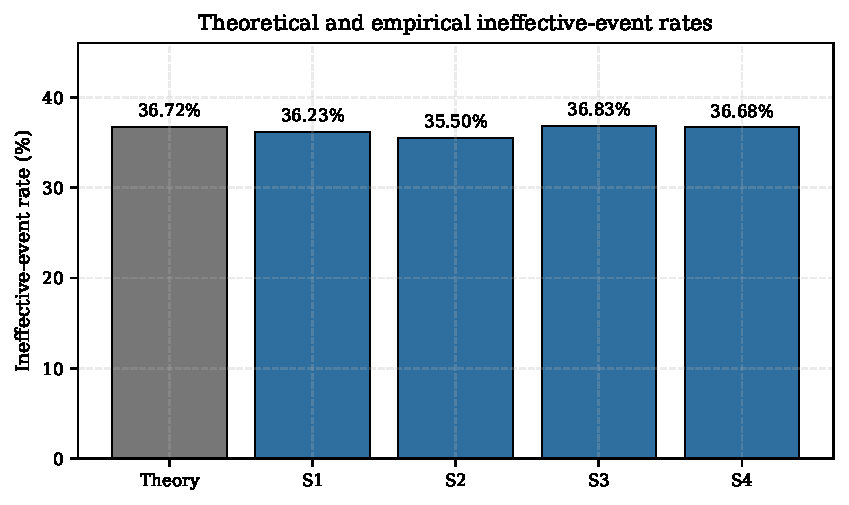
\includegraphics[width=\columnwidth]
    {paper_artifacts/figures/ineffective_rate_comparison.pdf}
    \caption{Comparison between the theoretical and empirical
    ineffective-event rates.}
    \label{fig:ineffective-rate}
\end{figure}

\begin{figure}[t]
    \centering
    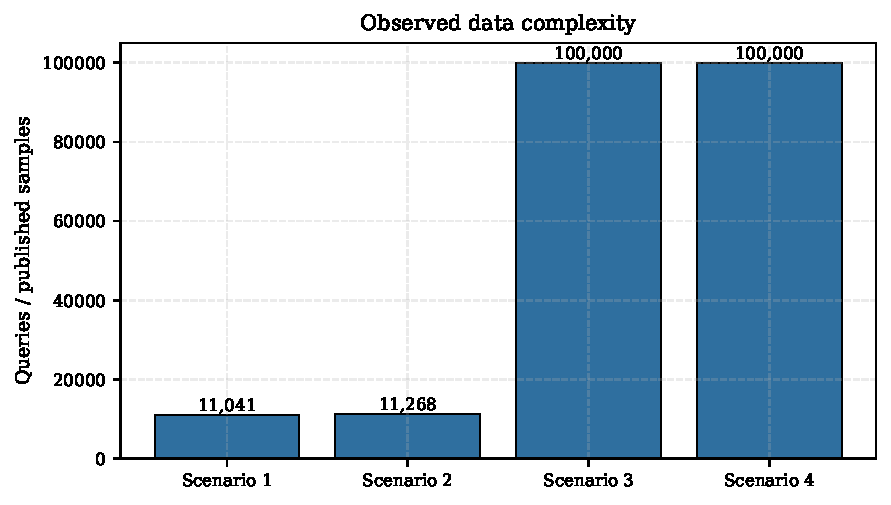
\includegraphics[width=\columnwidth]
    {paper_artifacts/figures/sample_complexity.pdf}
    \caption{Observed query or published-sample complexity of the
    evaluated SIPFA scenarios.}
    \label{fig:sample-complexity}
\end{figure}

\begin{figure*}[t]
    \centering
    \includegraphics[width=0.92\textwidth]
    {paper_artifacts/figures/scenario4_sei_all_candidates.pdf}
    \caption{Aggregate SEI score over all 256 fault-input candidates
    in Scenario~4.}
    \label{fig:scenario4-all-sei}
\end{figure*}

\begin{table*}[t]
\centering
\caption{Summary of the four SIPFA scenarios on Lilliput-TBC-II-128.}
\label{tab:scenario-summary}
\small
\begin{tabular}{clllrrrr}
\toprule
Scenario & Fault & Countermeasure & Method & Samples & Ineff. & Rate & Status \\
\midrule
1 & Known & Detection-based & Missing-value analysis & 11,041 & 4,000 & 36.23\% & PASS \\
2 & Unknown & Detection-based & Candidate filtering & 11,268 & 4,000 & 35.50\% & PASS \\
3 & Known & Infection-based & Minimum histogram & 100,000 & 36,829 & 36.83\% & PASS \\
4 & Unknown & Infection-based & SEI ranking & 100,000 & 36,681 & 36.68\% & PASS \\
\bottomrule
\end{tabular}
\end{table*}


\begin{table}[t]
\centering
\caption{Recovered secret-dependent values.}
\label{tab:recovered-values}
\small
\begin{tabular}{cll}
\toprule
Scenario & Recovered fault input & Recovered RTK[31] \\
\midrule
1 & 0x5a & \texttt{b3ed58adabab101d} \\
2 & 0x5a & \texttt{b3ed58adabab101d} \\
3 & Known / not recovered & \texttt{b3ed58adabab101d} \\
4 & 0x5a & \texttt{b3ed58adabab101d} \\
\bottomrule
\end{tabular}
\end{table}


% If Scenario 3 results are available:
% \begin{table}[t]
\centering
\caption{Lane-wise recovery results for Scenario 3.}
\label{tab:scenario3-lanes}
\small
\begin{tabular}{crrrrr}
\toprule
Lane & Min. bin & Min. count & Gap & Recovered RTK & Status \\
\midrule
0 & -- & 259 & 84 & 0xb3 & PASS \\
1 & -- & 251 & 91 & 0xed & PASS \\
2 & -- & 252 & 76 & 0x58 & PASS \\
3 & -- & 233 & 101 & 0xad & PASS \\
4 & -- & 251 & 94 & 0xab & PASS \\
5 & -- & 271 & 74 & 0xab & PASS \\
6 & -- & 243 & 83 & 0x10 & PASS \\
7 & -- & 253 & 85 & 0x1d & PASS \\
\bottomrule
\end{tabular}
\end{table}


% If Scenario 4 candidates are available:
% \input{paper_artifacts/tables/scenario4_top_candidates.tex}
